\section{\strace{} in Aktion}

\subsection{Analyse eines einfachen Programms}

\begin{frame}[t,fragile]
  \frametitle{Beispielhafte Analyse eines Python-Programms}

  \begin{lstlisting}
% strace notfound.py > output.txt
  \end{lstlisting}

  \centering
  \begin{columns}
    \column{\dimexpr\paperwidth}
    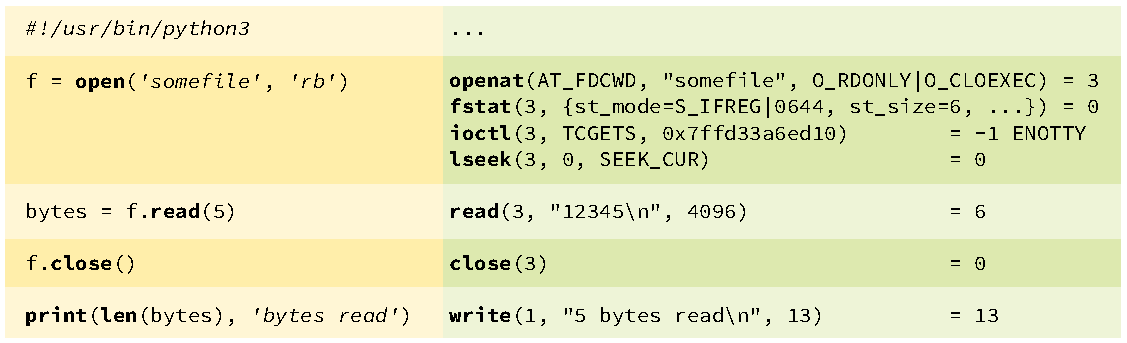
\includegraphics[width=\paperwidth]{../images/sample-listing.pdf}
  \end{columns}

\end{frame}

\begin{frame}[fragile]
  \frametitle{Fehlerfall}

  \begin{lstlisting}
% rm somefile
% strace notfound.py > output.txt
  \end{lstlisting}

  \begin{exampleblock}{\vspace*{-2ex}}
  \begin{lstlisting}
...
openat(AT_FDCWD, "somefile", O_RDONLY|O_CLOEXEC) =
   -1 ENOENT (Datei oder Verzeichnis nicht gefunden)
...
  \end{lstlisting}
  \end{exampleblock}


\end{frame}

\subsection{Kindprozesse und Threads}

\begin{frame}[fragile]
  \frametitle{Kindprozesse und Threads}

  \begin{block}{Prozesse und Threads}
    \begin{itemize}
      \item Kernel behandelt Threads und Prozesse erstmal ähnlich (als Scheduling-Einheit)
      \item Threads innerhalb des gleichen Prozesses haben gleiche PID aber andere TID
      \item \strace{} zeigt eigentlich die TID an, nennt das aber PID
     \end{itemize}
  \end{block}

  \begin{exampleblock}{Beispiel: \texttt{strace -f \ldots}}
    \begin{lstlisting}
clone(child_stack=0x7f4e991b0fb0, flags=CLONE_VM|CLONE_FS|CLONE_FILES|CLONE_SIGHAND|CLONE_THREAD|CLONE_SYSVSEM|CLONE_SETTLS|CLONE_PARENT_SETTID|CLONE_CHILD_CLEARTID, parent_tid=[40447], tls=0x7f4e991b1700, child_tidptr=0x7f4e991b19d0) = 40447
strace: Process 40447 attached
[pid 40447] set_robust_list(0x7f4e991b19e0, 24) = 0
[pid 40447] getpid()                    = 40446
          \end{lstlisting}
    \end{exampleblock}
\end{frame}

\subsection{Protokollierung in eine Datei}

\begin{frame}[fragile]
  \frametitle{Protokollierung in eine Datei}

  \vspace{-1mm}

  \begin{lstlisting}
    % strace -o DATEINAME
  \end{lstlisting}

  \vspace{-1mm}

  \begin{block}{Vorteile}
    \begin{itemize}
      \item Ausgabe von Programm und \strace{} klar getrennt
      \item Suchfunktion
      \item ggf. Syntax-Highlighting (vim)
     \end{itemize}
  \end{block}

  \begin{block}{Mehrere Prozesse}
    \begin{itemize}
      \item mit  Option \texttt{-ff} statt \texttt{-f}
         wird pro Kindprozess wird eigene Datei erstellt
      \item Namensschema \texttt{\emph{Dateiname.}PID}
     \end{itemize}
  \end{block}

  \begin{block}{Zeitstempel}
    \begin{itemize}
      \item \texttt{-t}: Sekunden-Genauigkeit
      \item \texttt{-tt}: Millisekunden-Genauigkeit
    \end{itemize}
  \end{block}
\end{frame}

\subsection{Filterfunktionen}

\begin{frame}[fragile]
  \frametitle{Filterfunktion: Einschränkung der Systemaufrufe}

  \begin{lstlisting}
    % strace -e trace=SET
    % strace -e trace=open,close # nur open und close
    % strace -e trace=%file      # Dateioperationen (Gruppe)
  \end{lstlisting}

  \begin{center}
    \begin{tabular}{|p{2cm}p{8.5cm}|}
      \hline
      \textbf{Gruppe} & \textbf{Operationen} \\
      \hline
      \texttt{\%file}          & Dateioperationen, die einen Dateinamen als Argument
                                bekommen, also beispielsweise \texttt{open,} \texttt{stat,}
                                \texttt{chmod,} \texttt{unlink,} … \\
      \texttt{\%desc}          & Dateioperationen, die einen Dateideskriptor als \newline
                                 Argument bekommen, also z.\,B. \texttt{read,} \texttt{write,}
                                \texttt{chmod,} \texttt{unlink,} … \\
      \texttt{\%process}       & Systemaurufe zur Prozessverwaltung \\
      \texttt{\%net}           & Systemaurufe zur Netzwerkprogrammierung \\
      \texttt{\%signal}        & Systemaurufe bzgl. Behandlung von Signalen \\
      \texttt{\%ipc}           & Operationen zur Interprozesskommunikation \\
      \texttt{\%memory}        & Systemaufrufe zur Speicherverwaltung \\
      \texttt{\%pure}          & Systemaufrufe ohne Argument, z.\,B. \texttt{getpid} \\
      \hline
    \end{tabular}
  \end{center}

\end{frame}



\subsection{Strings (Zeichenketten)}

\begin{frame}[fragile]
  \frametitle{Strings}

  \begin{itemize}
    \item Strings werden standardmäßig ab 50 Zeichen abgeschnitten
    \item mit der Option \texttt{-s \emph{LÄNGE}} kann Limit erhöht werden
    \item Dateinamen werden immer vollständig ausgegeben
  \end{itemize}

\end{frame}


\subsection{\strace{} einschränken}


\subsection{Strings}
